\begin{frame}{Motivación}
\small
\begin{block}{Ecuaciones diferenciales en la ciencia}
En la ciencia se pueden encontrar diferentes ecuaciones que modelan ciertos fenómenos de la física:\pause
\begin{itemize}
\item Crecimiento exponencial: \textbf{$\dfrac{dy}{dx}=ky$}
\item Ley de enfriamiento de Newton: \textbf{$\dfrac{dy}{dx}=k(A-y)$}
\item Vibraciones mecánicas: \textbf{$m\dfrac{d^2y}{dx^2}+c\dfrac{dy}{dx}
+ky=f(x)$}
\item Problema de los $N$ cuerpos (\textbf{Sistemas}): \textbf{$\dfrac{d^2y_i}{dx^2}=G\sum_{j=1,j\neq i}^{N}\dfrac{m_j}{|y_j-y_i|^3}(y_j-y_i)$}
\end{itemize}
\end{block}\pause
\begin{block}{Ecuación diferencial ordinaria lineal}
Una ecuación diferencial se dice lineal si esta se puede expresar como:
$$L(y)=b(x).$$
Donde $L$ es de la forma:
$$a_n(x)\dfrac{d^n}{dx^n}+a_{n-1}(x)\dfrac{d^{n-1}}{dx^{n-1}}+\cdots+a_0(x).$$
\end{block}
\end{frame}
\begin{frame}{Clasificación}
Si la ecuación diferencial no se puede escribir como en la definición anterior, entonces se dice que es una ecuación de diferencial no lineal. Un ejemplo de una ecuación diferencial no lineal se muestra a continuación:
$$y''y'+xy=0.$$
\begin{block}{Orden}
Se dice que una ecuación diferencial es de orden $n$ si la derivada más alta en la ecuación es de orden $n$.
\end{block}\pause
\begin{itemize}
\item $3x+y=y'$ (Orden 1, lineal).
\item $3xyy''+y'=0$ (Orden 2, no lineal).
\end{itemize}
\begin{block}{Proposición}
Toda ecuación diferencial de orden $n$ puede ser expresado como un sistema de ecuaciones diferenciales de primer orden. 
\end{block}
\end{frame}
\begin{frame}
\small
\begin{block}{Ejemplo}
Considere la ecuación diferencial no lineal de segundo orden:
$$3xyy''+y'=0.$$
Muestre que esta ecuación se puede plantear como un sistema de ecuaciones de primer orden.
\end{block}
Si se hace $y_0=y$ y $y_1=y'$, entonces el problema se puede plantear de la siguiente forma:
\begin{displaymath}
\left \{
\begin{array}{c}
y_1=y_0'\\
3xy_0y_1'+y_0'=0
\end{array}
\right.
\end{displaymath}
Esto se puede reescribir como:
\begin{displaymath}
\left(
\begin{array}{cc}
1 & 0\\
1 & 3xy_0
\end{array}
\right)
\left(
\begin{array}{c}
y_0'\\
y_1'
\end{array}
\right)=
\left(
\begin{array}{c}
y_1\\
0
\end{array}
\right)
\end{displaymath}
Esto a su vez se puede escribir en la forma:
\begin{displaymath}
\left(
\begin{array}{rr}
1 & 0\\
-\frac{1}{3xy_0} & \frac{1}{3xy_0}
\end{array}
\right)
\left(
\begin{array}{c}
y_1\\
0
\end{array}
\right)=
\left(
\begin{array}{c}
y_0'\\
y_1'
\end{array}
\right)
\end{displaymath}
$$Y=f(x,Y).$$
Donde $Y=(y_0,y_1).$
\end{frame}
\begin{frame}{Existencia y unicidad}
\small
\begin{block}{Ejemplo (Infinitas soluciones)}
Considere el problema de valor inicial:
$$y'=|y|^\alpha. \alpha\in (0,1)$$
$$y(0)=0.$$
Muestre que para cualquier $c$ positiva, la función $y_c(x)$ es una solución al problema de valor inicial:
\begin{displaymath}
y_c(x)=\left \{
\begin{array}{ll}
(1-\alpha)^{\dfrac{1}{1-\alpha}}(x-c)^{\dfrac{1}{1-\alpha}} & x\in [c,\infty[\\
0 & x\in [0,c[
\end{array}
\right.
\end{displaymath}
\end{block}
\end{frame}
\begin{frame}{Existencia y unicidad}
\textcolor{cyan}{
Suponga que $x>c$:
\begin{align*}
\dfrac{d}{dx}\bigg((1-\alpha)^{\dfrac{1}{1-\alpha}}(x-c)^{\dfrac{1}{1-\alpha}}\bigg)=&\bigg((1-\alpha)^{\dfrac{\alpha}{1-\alpha}}(x-c)^{\dfrac{\alpha}{1-\alpha}}\bigg)\\
=&|y_c(x)|^{\alpha}.
\end{align*}
Si $x<c$:
\begin{align*}
\dfrac{d}{dx}(0)=&|0|^\alpha.
\end{align*}
Finalmente en el caso $x=c$:
\begin{align*}
y_c'(c)=\lim_{h\rightarrow 0}\dfrac{f_c(c+h)-f_c(c)}{h}=0=|y_c(c)|^\alpha
\end{align*}\pause
Se puede probar que si $\alpha\geq 1$ entonces la solución es única. 
}
\end{frame}
\begin{frame}{Existencia y unicidad}
\begin{block}{Condición de Lipschitz}
Una función $f:[a,b]\times \mathbb{R}\rightarrow \mathbb{R}$ se dice de Lipschitz en la segunda variable si existe una constante positiva $L$ (conocida como constante de Lipschitz) y se verifica la siguiente desigualdad:
$$|f(x,u)-f(x,v)|\leq L|u-v|$$
para todo $u$, $v$ en los reales y para todo $x\in [a,b]$. 
\end{block}
\begin{block}{Teorema de existencia y unicidad}
Sean $D=[a,b]\times \mathbb{R}$ y $f:D\rightarrow \mathbb{R}$ continua. Suponga que $f$ satifasce la condición de Lipschitz en la segunda variable; entonces el problema de valor inicial $\dfrac{dy}{dx}=f(x,y)$, $y(a)=y_0$ tiene solución única.
\end{block}
\end{frame}
\begin{frame}
\begin{Def}[Conjunto Convexo]
Un conjunto $D$ es convexo si para cualesquiera $x$, $y$ en $D$ se tiene que $$\lambda x+(1-\lambda )y\in D.$$
\end{Def}
\begin{Teo}[Criterio]
Sea $f(t,y)$ definida en un conjunto convexo $D\subset \mathbb{R}^2.$ Si existe una constante $L>0$ con:
$$\bigg|\dfrac{\partial f}{\partial y}(t,y)\bigg|\leq L$$
entonces $f$ satisface una condición de Lipschitz en $D$ en la variable $y$ con la constante $L$ de Lipschitz.
\end{Teo}
\end{frame}
%====================================
\begin{frame}{Partición del intervalo}
\small
Una partición del intervalo $[a,b]$ de tamaño de paso $h>0$ es un conjunto de puntos $\{x_i\}_{i=0}^{N}$ donde $x_i=x_{i-1}+h$ para $i=1,\cdots, N.$ y $h=\dfrac{b-a}{N}$, $x_0=a$ y $x_N=b$.
\begin{block}{Partición de un intervalo}
\centering
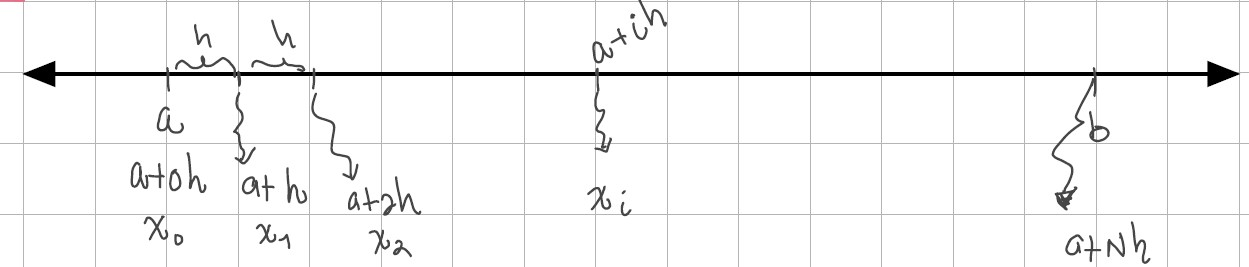
\includegraphics[scale=0.5]{TerceraUnidad/Imagen13}
\end{block}
\textcolor{red}{
De la definición anterior se puede ver que $x_k=a+kh$ para $k=0,\cdots, N$.}
\end{frame}

%=============================
\begin{frame}
\begin{block}{Partición del intervalo con $N$ puntos}
Suponga que se quiere tener $N$ puntos de aproximación en $[a, b]$ a una distancia $h$ entre cada dos puntos. Entonces, la partición del intervalo se hará  con 
$$t_i=a+jh \text{ tal que } h=\frac{b-a}{N}$$
\end{block}
Ejemplos:
\begin{enumerate}
\item Si se tiene el intervalo $[0, 3]$ y se quieren tener 15 puntos, entonces, la distancia entre cada dos puntos será:
$$h=\frac{3-0}{15}=\frac{1}{5}=0.2$$
\item Considere que se tiene el intervalo $[1, 4]$ y se hará una partición del intervalo con una distancia entre dos puntos $h=0.3$.  Entonces, la cantidad de puntos en la partición será:
$$N=\frac{4-1}{0.3}=10$$
\end{enumerate}
\end{frame}

%====================================
\begin{frame}{Métodos de un solo paso}
\begin{block}{Método de un solo paso explícito}
Un \textit{método de un solo paso explícito} es un método numérico en el que se aproximan las soluciones a un problema de valor inicial con la siguiente estructura:
$$w_k=w_{k-1}+h\phi(x_k,w_k;h)$$
donde $x_k$ (Como se definio arriba) representa los elementos en un partición y $w_k\approx y_k=y(x_k)$.
\end{block}
\end{frame}

%====================================
\begin{frame}{Método de Euler}
\textbf{Deducción de método de Euler: }
\textcolor{red}{
\begin{displaymath}
\begin{array}{rl}
y_{k+1}=&y(x_{k+1})\\\pause
=&y(x_k+h)=y(x_k)+hy'(x_k)+h^2/2y''(\xi)\\\pause
=&y_k+hf(y_k,x_k)+h^2/2y''(\xi)
\end{array}
\end{displaymath}}\pause
\begin{block}{Método de Euler}
El método de Euler consiste en generar los valores $\{w_k\}$ de manera tal que:
\begin{align*}
w_{k+1}&=w_{k}+hf(x_k,w_k)
\end{align*}
para $k=0,\cdots,N$.
\end{block}
En este caso las $w_k$ intentan aproximar a las $y_k$.
\end{frame}
\begin{frame}{Error del método de Euler}
\begin{block}{Teorema}
Considere las siguientes hipótesis:
\begin{itemize}
\item $f$ es continua en $D=[a,b]\times \mathbb{R}$.
\item $f$ satisface la condición de Lipschitz con constante $L$.
\item Existe una constante $M$ con la propiedad $|y''(x)|\leq M$ en $[a,b]$.
\item Sea $y$ la solución única del problema de valor inicial:
$$y'=f(x,y)$$
y con $y(a)=y_0.$ 
\item Sea  $\{w_k\}_{k=0}^{N}$ la sucesión generada por el método de Euler.
\end{itemize}
Entonces:
$$|y(x_k)-w_k|\leq \dfrac{hM}{2L}[\exp(L(x_k-a))-1]$$
\end{block}
\textbf{Observación: }\textcolor{red}{Note que la cota de error en la estimación anterior es lineal en $h$.}
\end{frame}
\begin{frame}{Errores de redondeo en el método de Euler}
Método de Euler considerando los errores de redondeo $\delta_k$:
\begin{displaymath}
\begin{array}{rl}
u_0=&a+\delta_0\\\pause
u_1=&u_0+hf(x_0,u_0)+\delta_1\\\pause
\vdots =&\vdots\\
u_{k+1}=&u_{k}+hf(x_k,u_k)+\delta_{k+1}\\\pause
\vdots =&\vdots\\
u_{N}=&u_{N-1}+hf(x_{N-1},u_{N-1})+\delta_{N}
\end{array}
\end{displaymath}
\end{frame}
\begin{frame}{Error del método de Euler con errores de redondeo}
\small
\begin{block}{Teorema}
Considere las siguientes hipótesis:
\begin{itemize}
\item $f$ es continua en $D=[a,b]\times \mathbb{R}$.
\item $f$ satisface la condición de Lipschitz con constante $L$.
\item Existe una constante $M$ con la propiedad $|y''(x)|\leq M$ en $[a,b]$.
\item Sea $y$ la solución única del problema de valor inicial:
$$y'=f(x,y)$$
y con $y(a)=y_0.$ 
\item Sea  $\{u_k\}_{k=0}^{N}$ la sucesión generada por el método de Euler con errores de redondeo.
\item $|\delta_k|\leq \delta$ para $\delta$ fijo. 
\end{itemize}
Entonces:
$$|y(x_k)-u_k|\leq \dfrac{1}{L}\bigg(\dfrac{hM}{2}+\dfrac{\delta}{h}\bigg)[\exp(L(x_k-a))-1]+|\delta_0|\exp(L(x_k-a)).$$
\end{block}
\textcolor{red}{Note que la cota de error ya no depende linealmente de $h$. De hecho posiblemente crece cuando $h$ se vuelve muy pequeño.}
\end{frame}
\begin{frame}{Errores de redondeo en el método de Euler.}
\small
Si se grafica la expresión $g(h)=\dfrac{hM}{2}+\dfrac{\delta}{h}$ se obtendría una gráfica como la siguiente:
\begin{figure}[H]
\centering 
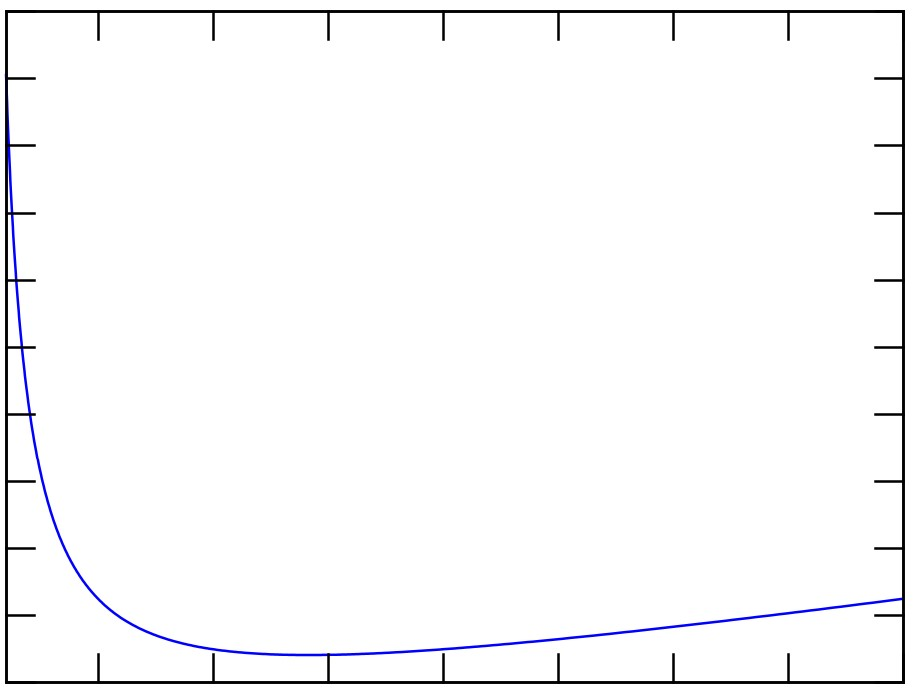
\includegraphics[scale=0.3]{TerceraUnidad/Imagen14}
\end{figure}
Se puede probar que el punto más bajo de esta grafica ocurre en $h=\sqrt{\dfrac{2\delta}{M}}$. Y se puede ver que esta cantidad crece cuando $h<\sqrt{\dfrac{2\delta}{M}}$. Entonces se puede imponer la condición de $h$ no sea mucho más pequeño que $\sqrt{\dfrac{2\delta}{M}}$. En la práctica esto es plausible dado que el error de redonde es considerablemente pequeño.
\section{Métodos de Taylor de orden superior}
\end{frame}
\begin{frame}{Métodos de Taylor de orden superior }
\begin{block}{Error local de truncamiento}
Considere el método de aproximación:
\begin{align*}
w_0=&y(x_0)\\
w_{k+1}=&w_k+h\phi(x_k,w_k)
\end{align*}
Se define el error local de truncamiento por:
$$\tau_{k+1}(h)=\dfrac{y_{k+1}-y_k}{h}-\phi(x_k,y_k)$$
Para $k=0,\cdots, N-1$.
\end{block}
\begin{block}{Notación O}
Se dice que  una función $f:A\subset\mathbb{R}\rightarrow \mathbb{R}^n$ es $O(h^p)$ si existe una constante positiva $M$ tal que  $f(h)\leq Mh^p$ para toda $h\in A$.
\end{block}
\textcolor{red}{En los métodos númericos para problemas de valor inicial se busca que $\tau_{k}(h)$ sea $O(h^p)$ para algún $p$ positivo.\\\pause }
\textcolor{cyan}{El método se considera de mejor orden de convergencia en tanto el valor de $p$ sea mas grande.}
\end{frame}
\begin{frame}{Ejemplo 1}
\begin{block}{Ejercicio teórico}
Pruebe que el método de Euler es un método  con un error de truncamiento $O(h)$ cuando su segunda derivada esta acotada por una constante $M$.
\end{block}
\begin{displaymath}
\begin{array}{rl}
\tau_{k+1}(h)=&\dfrac{y_{k+1}-y_k}{h}-\phi(x_k,y_k)\\\pause
=&\dfrac{y_{k+1}-y_k}{h}-f(x_k,y_k)\\\pause
=&\dfrac{y(x_{k+1})-y(x_k)}{h}-f(x_k,y(x_k))\\\pause
=&\dfrac{y(x_{k}+h)-y(x_k)}{h}-y'(x_k)\\\pause
=&\dfrac{y(x_{k})+hy'(x_k)+h^2/2y''(\xi)-y(x_k)}{h}-y'(x_k)\\\pause
=&y'(x_k)+h/2y''(x_k)-y'(x_k)\\\pause
\leq & hM/2\\\pause
\in & O(h).
\end{array}
\end{displaymath}
\end{frame}
\begin{frame}{Métodos de orden superior}
\begin{block}{Método de Taylor de orden $n$}
El método de Taylor de orden $n$ para un problema de valor inicial se define como:
\begin{align*}
w_0&=\alpha\\
w_{k+1}&=w_k+hT^{(n)}(x_k,w_k)\\
&=w_k+h\bigg[f(x_k,w_k)+\dfrac{h}{2}[\dfrac{d}{dx}f(x_k,w_k)]+\cdots +\dfrac{h^{n-1}}{n!}\dfrac{d^{n-1}}{dx^{n-1}}[f(x_k,w_k)\bigg]
\end{align*}
\end{block}
\begin{block}{Teorema}
Si se utiliza el método de Taylor de orden $n$ con paso $h$ para aproximar la solución  del problema de valor incial:
\begin{itemize}
\item $y(x_0)=y_0$
\item $y'(x)=f(x,y)$
\item $x\in[a,b]$
\item $y\in C^{n+1}[a,b]$
\end{itemize}
Entonces el error de truncamiento es $O(h^n)$.
\end{block}
\end{frame}
\begin{frame}{Método de Taylor de orden $n$}
\begin{block}{Ejercicios}
Aplique el método de Taylor de orden 3 para aproximar la solución del problema de valor incial:
\begin{itemize}
\item $y(0)=1$, $h$=0.25
\item $y'(x)=-xy+4x/y$. $x\in[0,1]$.
\end{itemize}
\end{block}
\textcolor{red}{
\begin{displaymath}
\begin{array}{rl}
\dfrac{df(x,y(x))}{dx}=&\dfrac{\partial f(x,y)}{\partial x}+\dfrac{\partial f(x,y)}{\partial y}y'(x)\\\pause
=&\dfrac{\partial f(x,y)}{\partial x}+\dfrac{\partial f(x,y)}{\partial y}f(x,y)\\\pause
=&x^2y-y+\dfrac{4}{y}-\dfrac{16x^2}{y^3}\\\pause
\dfrac{d^2f(x,y(x))}{dx^2}=&f_{xx}+2ff_{xy}+f^2f_{yy}+f_xf_y+f_y^2f\\\pause
=&\displaystyle{{8\,{\it xy}}\over{y^2}}+{{8\,x\,{\it xy}^2}\over{y^3}}-{{48\,x
 }\over{y^3}}-{{80\,x^2\,{\it xy}}\over{y^4}}+{{192\,x^3}\over{y^5}}\\
\end{array}
\end{displaymath}
}
\end{frame}
\begin{frame}{Método de Taylor de orden 3}
\small
\textcolor{cyan}{
\begin{displaymath}
\begin{array}{rl}
T^{(3)}(x,y)=&f(x,y)+\dfrac{h}{2}[\dfrac{d}{dx}f(x,y)]+\dfrac{h^{2}}{3!}\dfrac{d^{2}}{dx^{2}}[f(x,y)].\\
=&\displaystyle {{\left(h\,x^2-2\,x-h\right)\,y^4+\left(8\,x+4\,h\right)\,y^2-16\,h
 \,x^2}\over{2\,y^3}}\\
 &\displaystyle -{{\left(h^2\,x^3-3\,h^2\,x\right)\,y^6-4\,h^2\,x^3\,y^4+\left(48\,
 h^2\,x^3+48\,h^2\,x\right)\,y^2-192\,h^2\,x^3}\over{6\,y^5}}
\end{array}
\end{displaymath}
}
Finalmente el método numérico queda expresado en la siguiente forma:
\textcolor{cyan}{
\begin{displaymath}
\renewcommand{\arraystretch}{1.5}
\begin{array}{rl}
w_{k+1}=&\displaystyle {\it w_k}-{{h\,\left({\it w_k}^2-4\right)\,{\it x_k}}\over{
 {\it w_k}}}+\\
 &\displaystyle {{h^2\,\left(\left({\it w_k}^4-16\right)\,{\it x_k}^2-{\it w_k}^
 4+4\,{\it w_k}^2\right)}\over{2\,{\it w_k}^3}}\\
 &\displaystyle -{{h^3\,\left(\left({\it w_k}^6-4\,{\it w_k}^4+48\,{\it w_k}^2-
 192\right)\,{\it x_k}^3+\left(48\,{\it w_k}^2-3\,{\it w_k}^6
 \right)\,{\it x_k}\right)}\over{6\,{\it w_k}^5}}
\end{array}
\end{displaymath}
}
\end{frame}
\begin{frame}{Soluciones numéricas del método de Taylor de orden 3}
\begin{table}[H]
\renewcommand{\arraystretch}{1.4}
\begin{tabular}{cccccc}
$k$&0&1&2&3&4\\\hline
$x_k$&0&0.25&0.5&0.75&1\\
$w_k$&1&1.125&1.3442&1.5693&1.7528\\\hline
\end{tabular}
\caption{Iteraciones del método de orden 3.}
\end{table}
\end{frame}
\begin{frame}{Solución numérica del método de Taylor de orden 3}
\begin{figure}[H]
\centering
\includegraphics[scale=0.8]{TerceraUnidad/Imagen15}
\end{figure}
\end{frame}	
%=============================
\section{Método de Runge-Kutta}
\begin{frame}{Método de Runge-Kutta}
Estudiaremos dos categorias de los métodos de Runge-Kutta:
\begin{enumerate}
\item Metodos de Runge-Kutta de orden 2, donde encontramos los métodos 
\begin{itemize}
\item Método de punto medio\\

\item Método de Euler modificado\\

\item Método de Heun
\end{itemize}
\item Metodos de Runge-Kutta de orden 4
\end{enumerate}
\end{frame}

%=============================
\begin{frame}{Métodos de Runge-Kutta de Orden 2}
\begin{block}{Método del punto medio}
\begin{align*}
w_0 &=\alpha,\\
w_{i+1}&=w_{i}+hf(t_i+\frac{h}{2}, w_i+\frac{h}{2}f(t_i, w_i))
\end{align*}
\hspace{3cm}para cada $i=0, 1, 2,...., N-1$
\end{block}
\end{frame}


%=============================
\begin{frame}{Ejemplo}
\begin{block}{Ejercicio tomado del libro de R. Burden, Sec. 5.4}
Resuelva aplicando el \textbf{método de punto medio} el problema de valor inicial
$$y'=1+(t-y)^2, \quad 2\leq t\leq 2.9 \quad y(2)=1, \quad N=7.$$
Además, estime el error $|w_i-y(t_i)|$ de las aproximaciones encontradas por medio de la solución real 
$$y=t+\dfrac{1}{1-t}$$
\end{block}
\begin{displaymath}
\begin{array}{r|lll}
i& t_i& w_i & |w_i-y(t_i)|\\
\hline\hline
0&2&1   &0\\
1&2.1286&1.2411 &0.0013519\\
2&2.2571&1.4597 &0.001943\\
3&2.3857&1.6619 &0.0021633\\
4&2.5143&1.8517 &0.002199\\
5&2.6429&2.032  &0.0021428\\
6&2.7714&2.2049 &0.002043\\
7&2.9&2.3718    &0.0019248\\
\end{array}
\end{displaymath}
\end{frame}
%=============================

\begin{frame}{Métodos de Runge-Kutta de Orden 2}
\begin{block}{Método de Euler Modificado}
\begin{align*}
w_0 &=\alpha,\\
w_{i+1}&=w_{i}+\frac{h}{2}[f(t_i, w_i)+f(t_i+h, w_i+hf(t_i, w_i))]
\end{align*}
\hspace{3cm}para cada $i=0, 1, 2,...., N-1$
\end{block}
\end{frame}

%=============================
\begin{frame}{Ejemplo}
\begin{block}{Ejercicio tomado del libro de R. Burden, Sec. 5.4}
Resuelva aplicando el \textbf{método de Euler modificado} el problema de valor inicial
$$y'=\cos(2t)+\sen(3t), \quad 0\leq t\leq 1 \quad y(0)=1, \quad N=7.$$
Además, estime el error $|w_i-y(t_i)|$ de las aproximaciones encontradas por medio de la solución real 
$$y=\frac{1}{2}sen(2t)-\frac{1}{3}cos(3t)+\frac{4}{3}$$
\end{block}
\begin{displaymath}
\begin{array}{r|lll}
i& t_i& w_i & |w_i-y(t_i)|\\
\hline\hline
0&0&1   &       0\\
1&0.14286&1.1696        &       0.0014228\\
2&0.28571&1.3819        &       0.0036097\\
3&0.42857&1.6113        &       0.0062533\\
4&0.57143&1.827 &       0.0089484\\
5&0.71429&1.9975        &       0.01126\\
6&0.85714&2.096 &       0.012797\\
7&1&2.1047      &       0.013281\\
\end{array}
\end{displaymath}
\end{frame}

%=============================
\begin{frame}{Métodos de Runge-Kutta de Orden 2}
\begin{block}{Método de Heun}
\begin{align*}
w_0 &=\alpha,\\
w_{i+1}&=w_{i}+\frac{h}{4}[f(t_i, w_i)+3f(t_i+\frac{2}{3}h, w_i+\frac{2}{3}hf(t_i, w_i))]
\end{align*}
\hspace{3cm}para cada $i=0, 1, 2,...., N-1$
\end{block}
\end{frame}

%=============================
\begin{frame}{Ejemplo}
\begin{block}{Ejercicio tomado del libro de R. Burden, Sec. 5.4}
Resuelva aplicando el \textbf{método de Heun} el problema de valor inicial
$$y'=1+\frac{y}{t}+(\frac{y}{t})^2, \quad 0\leq t\leq 3 \quad y(1)=0, \quad N=7.$$
Además, estime el error $|w_i-y(t_i)|$ de las aproximaciones encontradas por medio de la solución real 
$$y=t\tan(lnt)$$
\end{block}
\begin{displaymath}
\begin{array}{r|lll}
i& t_i& w_i & |w_i-y(t_i)|\\
\hline\hline
0&1&0   &       0\\
1&1.2857&0.32549        &       0.0046118\\
2&1.5714&0.7502 &       0.012739\\
3&1.8571&1.2968 &       0.026327\\
4&2.1429&1.9965 &       0.048909\\
5&2.4286&2.895  &       0.086822\\
6&2.7143&4.0616 &       0.15195\\
7&3&5.6061      &       0.26802\\
\end{array}
\end{displaymath}
\end{frame}

%=============================
\begin{frame}{Gráficas de la solución y su aproximación}
A continuación se muestra una gráfica que presenta la aproximación obtenida usando el método de punto medio, método de Euler modificado y el método de Heun, de izquierda a derecha.
\begin{figure}
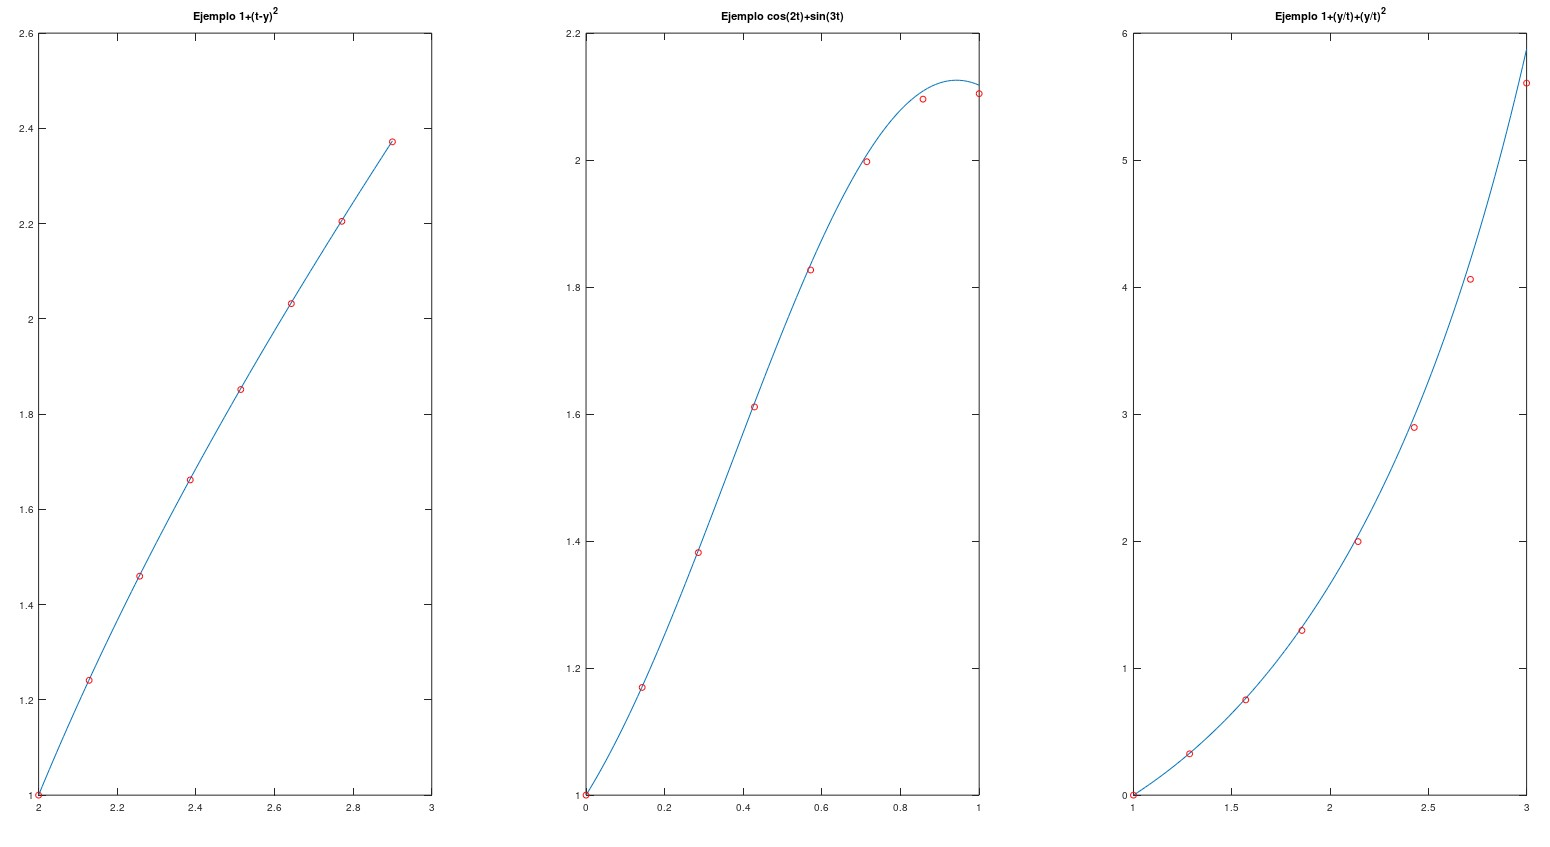
\includegraphics[scale=0.4]{TerceraUnidad/GraficaApro_RungeKutta}
\caption{La solución real está graficada con una linea continua y la aproximación por medio de los puntos rojos}
\end{figure}
\end{frame}

%=============================
\begin{frame}{Método de Runge-Kutta de orden 4}
\begin{block}{Método}
\begin{align*}
w_0 &= \alpha\\
k_1 &=hf(t_i, w_i)\\
k_2 &=hf(t_i+\frac{h}{2}, w_i+\frac{1}{2}k_1)\\
k_3 &=hf(t_i+\frac{h}{2}, w_i+\frac{1}{2}k_2)\\
k_4 &=hf(t_{i+1}, w_i+k_3)\\
w_{i+1}&=w_i+\frac{1}{6}(k_1+2k_2+2k_3+k_4)
\end{align*}
\hspace{3cm}para cada $i=0, 1, 2,...., N-1$
\end{block}
\end{frame}
%=============================
\begin{frame}{Método de Runge-Kutta para sistema de ecuaciones}
Sea $w_{ij}$ una aproximación de $u_i(t_i)$ para cada $j=0, 1, 2,..., N$ y  cada $i=1, 2, ...., m$ del sistema de ecuaciones diferenciales de primer orden con valor inicial:
\begin{align*}
\frac{du_1}{dt}&=f_1(t, u_1, u_2,... u_m),\\
\frac{du_2}{dt}&=f_2(t, u_1, u_2,... u_m),\\
\vdots\\
\frac{du_m}{dt}&=f_m(t, u_1, u_2,... u_m),\\
\end{align*} 
tal que $a\leq t \leq b$ y satisface las condiciones iniciales: 
$$u_1(a)=\alpha_1, u_2(a)=\alpha_2,\hdots, u_m(a)=\alpha_m$$
\end{frame}



%====================================
\begin{frame}
Sean $w_{10}=\alpha_1$, $w_{20}=\alpha_2$, ..., $w_{m0}=\alpha_m$ las condiciones iniciales del sistema de ecuaciones. 
\begin{block}{Definción del método}
Para $i$ fijo en cada iteración, con $j=0, 1, \hdots, N$ y con $i=1, 2, ..., m$
\begin{align*}
k_{1i} &= hf_i(t_j, w_{10}, w_{20}, \hdots, w_{m0}),\\
k_{2i} &= hf_i(t_i+\frac{1}{2}h, w_{1j}+\frac{1}{2}k_{11}, w_{2j}+\frac{1}{2}k_{12}, \hdots, w_{mj}+\frac{1}{2}k_{1m} ),\\
k_{3i} &= hf(t_i+\frac{1}{2}h, w_{1j}+\frac{1}{2}k_{21}, w_{2j}+\frac{1}{2}k_{22}, \hdots, w_{mj}+\frac{1}{2}k_{2m} ),\\
k_{4i}&=hf_i(t_i+h, w_{1j}+k_{31}, w_{2j}+k_{32}, \hdots, w_{mj}+k_{3m}),\\
w_{i(j+1)}&= w_{ij}+\frac{1}{6}(k_{1i}+2k_{2i}+2k_{3i}+k_{4i})
\end{align*} 
\end{block}
\end{frame}

%===================================
\subsection{Ejemplos}
\begin{frame}{Ejemplo 1}
\begin{block}{Ejericio tomado del libro de R. Burden, Sec. 5.9, 2.c}
Utilice el método de Runge-Kutta para sistemas de ecuaciones diferenciales para encontrar la aproximación de 
$$y'''+2y''-y'-2y=e^t$$
en $0 \leq t \leq 3$ y $h=0.2$. \\
Considere las condiciones iniciales $y(0)=1$, $y'(0)=2$, $y''(0)=0$.\\
\end{block}

\vspace{1cm}
Introducimos la variable $u_i(t)$ para generar el sistema de ecuaciones de primer orden deseado, entonces:
\begin{align*}
u_1(t) &= y(t),\\
u_2(t) &= y'(t),\\
u_3(t) &= y''(t),
\end{align*}
\end{frame}


\begin{frame}
Por lo tanto, se obtiene el siguiente sistema:
\begin{align*}
u_1' &= u_2,\\
u_2' &= u_3,\\
u_3' &= e^t+2u_1+u_2-2u_3
\end{align*}

Para aplicar el método, introducimos las variables de aproximación $w_{ij}$, se definen las condiciones iniciales asi:
\begin{align*}
w_{10} &= u_1(0)=1,\\
w_{20} &= u_2(0)=2,\\
w_{30} &= u_3(0)=0
\end{align*}

 Además se definen las funciones $f_i$ como sigue
 \begin{align*}
 f_1(t, w_1, w_2, w_3)&=w_2,\\
 f_2(t, w_1, w_2, w_3)&=w_3,\\
 f_3(t, w_1, w_2, w_3)&=e^t+2w_1+w_2-2w_3,\\
 \end{align*}
\end{frame}

%====================================
\begin{frame}{Iteración 1 $(i=1, j=1)$}
Haciendo los respectivos cálculos se obtiene:
\begin{align*}
k_{11} &= hf_1(t_0, w_{10}, w_{20}, w_{30})=0.4\\
k_{12} &= hf_2(t_0, w_{10}, w_{20}, w_{30})=0\\
k_{13} &= hf_3(t_0, w_{10}, w_{20}, w_{30})=1\\
k_{21} &=hf_1(t_0 +\frac{1}{2}h, w_{10}+\frac{1}{2}k_{11}, w_{20}+\frac{1}{2}k_{12}, w_{30}+\frac{1}{2}k_{13})=0.4\\
k_{22} &=hf_2(t_0 +\frac{1}{2}h, w_{10}+\frac{1}{2}k_{11}, w_{20}+\frac{1}{2}k_{12}, w_{30}+\frac{1}{2}k_{13})=0.1\\
k_{23} &=hf_3(t_0 +\frac{1}{2}h, w_{10}+\frac{1}{2}k_{11}, w_{20}+\frac{1}{2}k_{12}, w_{30}+\frac{1}{2}k_{13})=0.901034\\
k_{31}&=hf_1(t_0+\frac{1}{2}h, w_{10}+\frac{1}{2}k_{21}, w_{20}+\frac{1}{2}k_{22}, w_{30}+\frac{1}{2}k_{23})=0.41\\
k_{32}&=hf_2(t_0+\frac{1}{2}h, w_{10}+\frac{1}{2}k_{21}, w_{20}+\frac{1}{2}k_{22}, w_{30}+\frac{1}{2}k_{23})=0.0901034\\
k_{33}&=hf_3(t_0+\frac{1}{2}h, w_{10}+\frac{1}{2}k_{21}, w_{20}+\frac{1}{2}k_{22}, w_{30}+\frac{1}{2}k_{23})=0.930827\\
\end{align*}
\end{frame}


%==============================================
\begin{frame}
\begin{align*}
k_{41} &= hf_1(t_0+h, w_{10}+k_{31}, w_{20}+k_{32}, w_{30}+k_{33})=0.41802068\\
k_{42} &= hf_2(t_0+h, w_{10}+k_{31}, w_{20}+k_{32}, w_{30}+k_{33})=0.1861654\\
k_{43} &= hf_3(t_0+h, w_{10}+k_{31}, w_{20}+k_{32}, w_{30}+k_{33})=0.853970
\end{align*}
Entonces, las estimaciones obtenidas en la primera iteración son:
\begin{align*}
w_{11}&=w_{10}+\frac{1}{6}(k_{11}+2k_{21}+2k_{31}+k_{41})=1.4063\\
w_{21}&=w_{20}+\frac{1}{6}(k_{12}+2k_{22}+2k_{32}+ k_{42})=2.0944\\
w_{31}&=w_{30}+\frac{1}{6}(k_{13}+2k_{23}+2k_{33}+ k_{43})=0.9196\
\end{align*}
\end{frame}

\begin{frame}{Todas las iteraciones del método}
\begin{table}[]
\renewcommand{\arraystretch}{1.5}
\begin{tabular}{|l|l|l|l|}
\hline
\textbf{i} & \textbf{$w_{1i}$} & \textbf{$w_{2i}$} & \textbf{$w_{3i}$} \\ \hline
0 & 1.0000 & 2.0000 & 0 \\ \hline
1 & 1.4063 & 2.0944 & 0.9196 \\ \hline
2 & 1.8492 & 2.3619 & 1.7472 \\ \hline
3 & 2.3619 & 2.7929 & 2.5676 \\ \hline
4 & 2.9776 & 3.3931 & 3.4501 \\ \hline
5 & 3.7316 & 4.1812 & 4.4572 \\ \hline
6 & 4.6646 & 5.1884 & 5.6503 \\ \hline
7 & 5.8244 & 6.4581 & 7.0951 \\ \hline
8 & 7.2691 & 8.0480 & 8.8658 \\ \hline
9 & 9.0698 & 10.0318 & 11.0500 \\ \hline
10 & 11.3142 & 12.5024 & 13.7530 \\ \hline
11 & 14.1109 & 15.5759 & 17.1030 \\ \hline
12 & 17.5943 & 19.3970 & 21.2580 \\ \hline
13 & 21.9314 & 24.1454 & 26.4122 \\ \hline
14 & 27.3290 & 30.0441 & 32.8060 \\ \hline
15 & 34.0440 & 37.3697 & 40.7362 \\ \hline
\end{tabular}
\end{table}
\end{frame}

%===============================
\begin{frame}{Ejemplo 2}
\begin{block}{Ejercicio tomado de un examen de reposición del IIPA2022}
Resuelva la ecuación diferencial 
$ty''+t^2y'+ty=e^t$ en  $1\leq t \leq 1.5$ con $y(1)=0$ y $y'(1)=1$. Usando el método de Runge-Kutta de orden 4 para sistemas de ecuaciones diferenciales. Tome $h=0.5$.
\end{block}

Introducimos el cambio de variable siguiente con el propósito de generar el sistema de ecuaciones diferenciales:
\begin{align*}
u_1 &=y\implies u_1'=y'\implies u_1'\implies u_2\\
u_2 &=y'
\end{align*}
Entonces, si se despeja para la segunda derivada en $ty''+t^2y'+ty=e^t$ y luego se sustituye $y$ y sus derivadas, se obtiene:
\begin{align*}
u_1' &= u_2\\
u_2' &= -u_1+tu_2+\frac{e^t}{t}\\
\end{align*}
Finalmente, definimos $f_1(t, u_1, u_2)=u_2$ y $f_2(t, u_1, u_2)=-u_1+tu_2+e^t/t$ 
\end{frame}

\begin{frame}{Iteración 1 $(i=1, j=1)$}
Dadas las condiciones iniciales se tiene que $t_0=1$, $u_1(1)=0=w_{10}$ y $u_2(1)=1=w_{20}$. Entonces, 
\begin{align*}
k_{11} &= hf_1(t_0, w_{10}, w_{20})=0.5\\
k_{12} &= hf_2(t_0, w_{10}, w_{20})=1.859141\\
k_{21} &= hf_1(t_0+\frac{1}{2}h, w_{10}+\frac{1}{2}k_{11}, w_{20}+\frac{1}{2}k_{12})=0.964785\\
k_{22} &= hf_2(t_0+\frac{1}{2}h, w_{10}+\frac{1}{2}k_{11}, w_{20}+\frac{1}{2}k_{12})=2.477119\\
k_{31} &= hf_1(t_0+\frac{1}{2}h, w_{10}+\frac{1}{2}k_{21}, w_{20}+\frac{1}{2}k_{22})=1.119280\\
k_{32} &= hf_2(t_0+\frac{1}{2}h, w_{10}+\frac{1}{2}k_{21}, w_{20}+\frac{1}{2}k_{22})=2.554041\\
k_{41} &= hf_1(t_0+h, w_{10} + k_{31}, w_{20}+k_{32})=1.777021\\
k_{42} &= hf_2(t_0+h, w_{10} + k_{31}, w_{20}+k_{32})=3.599787\\
w_{11}&=w_{10}+\frac{1}{6}(k_{11}+2k_{21}+2k_{31}+k_{41})=1.0742\\
w_{21}&=w_{20}+\frac{1}{6}(k_{21}+2k_{22}+2k_{32}+k_{42})=3.5869\\
\end{align*}
\end{frame}

%================================
\begin{frame}{Tabla de iteraciones para $1\leq t \leq 5$}
\begin{table}[]
\renewcommand{\arraystretch}{1.5}
\begin{tabular}{|l|l|l|}
\hline
\textbf{i} & \textbf{$w_{1i}$} & \textbf{$w_{2i}$} \\ \hline
0 & 0 & 1.0000 \\ \hline
1 & 1.0742 & 3.5869 \\ \hline
2 & 4.1150 & 9.5110 \\ \hline
3 & 1.2320e+01 & 2.6704e+01 \\ \hline
4 & 3.7590e+01 & 8.9199e+01 \\ \hline
5 & 1.3384e+02 & 3.7509e+02 \\ \hline
6 & 6.0344e+02 & 2.0257e+03 \\ \hline
7 & 3.5549e+03 & 1.4028e+04 \\ \hline
8 & 2.7261e+04 & 1.2333e+05 \\ \hline
\end{tabular}\\
\vspace{1cm}
Nota: la notación e+$\alpha$, denota una potencia de 10, es decir
$$1.2320e+01=1.2320\times 10^{01}=1.2320\times 10=12.320$$
\end{table}
\end{frame}

%====================================
\section{Método de diferencias finitas,sitemas EDO orden 2}
\begin{frame}{Deducción del método}
\begin{block}{Problema}
Se desea encontrar una aproximación por el método de diferencias finitas para el problema de valor en la frontera de segundo orden
$$y''=p(x)y'+q(x)y+r(x)$$
para $a\leq x\leq b$, con las condiciones en la frontera $y(a)=\alpha$ y $y(b)=\beta$
\end{block}

\textbf{Región de aproximación}\\
La aproximación se hará en una partición del intervalo $[a, b]$ en $N+1$ intervalos, tal que :
\begin{itemize}
\item Los extremos de los intervalos de la partición son los puntos $x_i=a+ih$.
\item  Todos los puntos $x_i$ estan separados a una distancia $h=\frac{b-a}{N+1}$
\end{itemize}
\end{frame}

%=================================
\begin{frame}{Recordando el polinomio de Taylor}
Suponga que $f \in C^n[a, b]$, que $f^{(n+1)}$ existe en $[a, b]$ y $x_0 \in [a, b]$. Para cada $x \in [a,b]$ existe un número $\xi(x)$ entre $x_0$ y $x$ tal que
$$f(x)=P_n(x)+R_n(x)$$
donde 
\begin{align*}
P_n(x)&=f(x_0)+f'(x_0)(x-x_0)+\frac{f''(x_0)}{2!}(x-x_0)^2+\hdots + \frac{f^{(n)}(x_0)}{n!}(x-x_0)^k\\
R_n(x) &=\frac{f^{(n+1)}(\xi(x))}{(n+1)!}(x-x_0)^{n+1}\\
\end{align*}
\end{frame}

%===================================
\begin{frame}{Polinomio de Taylor para diferencias finitas}
\begin{enumerate}
\item Se desarrolla el tercer polinomio de Taylor
$$P_3(x)=f(x_0)+f'(x_0)(x-x_0)+\frac{f''(x_0)}{2!}(x-x_0)^2+\frac{f'''(x_0)}{3!}(x-x_0)^3$$
\item Se sustituye $y(x)=f(x)$ y se evalua en $x_i$
$$P_3(x)=y(x_i)+y'(x_i)(x-x_i)+\frac{y''(x_i)}{2!}(x-x_i)^2+\frac{y'''(x_i)}{3!}(x-x_i)^3$$
\item Se evalua en $x_{i+1}$ tomando en cuenta que $x_{i+1}=x_i+h$
\begin{align*}
y(x_{i+1})&=y(x_i)+y'(x_i)((x_i+h)-x_i)\\
&+\frac{y''(x_i)}{2!}((x_i+h)-x_i)^2+\frac{y'''(x_i)}{3!}((x_i+h)-x_i)^3\\
&=y(x_i)+hy'(x_i)+\frac{h^2}{2}y''(x_i)+\frac{h^3}{6}y'''(x_i)
\end{align*}
\item Se evalua en $x_{i-1}$ con $x_{i-1}=x_i-h$
$$y(x_{i-1})=y(x_i)-hy'(x_i)+\frac{h^2}{2}y''(x_i)-\frac{h^3}{6}y'''(x_i)$$
\end{enumerate}
\end{frame}


%===================================
\begin{frame}
Sumando las ecuaciones anteriores se obtiene
$$y(x_{i+1})+y(x_{i-1})=2y(x_i)+h^2y''(x_i)$$
Finalmente, se despeja para $y''(x_i)$ para obtener la aproximación en diferencias para la segunda derivada:
\begin{equation}
y''(x_i)=\frac{y(x_{i+1})-2y(x_i)+y(x_{i-1})}{h^2}
\label{SegundaDerivadaDiferencias}
\end{equation}

De manera similar se puede obtener la aproximación para la primera derivada 
\begin{equation}
y'(x_i)= \frac{y(x_{i+1})-y(x_{i+1})}{2h}
\label{PrimeraDerivadaDiferencias}
\end{equation}
\end{frame}

%====================================
\begin{frame}
Tomando la ecuación del problema inicial 
$$y''=p(x)y'+q(x)y+r(x)$$
y sustituyendo \eqref{SegundaDerivadaDiferencias} y \eqref{PrimeraDerivadaDiferencias}, se obtiene
\begin{align*}
\frac{y(x_{i+1})-2y(x_i)+y(x_{i-1})}{h^2}  &=
p(x_i)\bigg[ \frac{y(x_{i+1})-y(x_{i+1})}{2h}\bigg]+q(x_i)y(x_i)+r(x_i)
\end{align*}

\begin{block}{Método de diferencias finitas con error de truncamiento de orden $O(h^2)$}
Para $i=1, 2, 3, \hdots, N$
$$\bigg[\frac{-w_{i-1}+2w_i-w_{i+1}}{h^2}\bigg]+p(x_i)\bigg[\frac{w_{i+1}-w_{i-1}}{2h}\bigg]+q(x_i)w_i=-r(x_i)$$
con las condiciones de frontera
$w_0=\alpha$ y $w_{N+1}=\beta$
\end{block}
\end{frame}

%=====================================
\begin{frame}
La ecuación anterior se puede reescribir así:
\begin{equation}
-\bigg[1+\frac{h}{2}p(x_i) \bigg]w_{i-1}+[2+h^2q(x_i)]w_{i}-\bigg[ 1-\frac{h}{2} p(x_{i}) \bigg]w_{i+1}=-h^2r(x_i)
\label{EcuacionDiferencias}
\end{equation}

\vspace{1cm}
La ecuación \eqref{EcuacionDiferencias} genera un sistema de ecuaciones lineales de la forma 
$$\mathbf{Aw=b}.$$
Donde $A$ es una matriz tridiagonal de $N\times N$ teniendo siempre a $N\geq 2$.\\
\vspace{1cm}
A continuación se descibirá la forma matricial del método de diferencias finitas. 
\end{frame}


%=====================================
\begin{frame}{Forma matricial del método de diferencias finitas}
\scriptsize
\begin{equation}
\mathbf{A}=\begin{pmatrix}
2+h^2q(x_1) & -1+\frac{h}{2}p(x_1) & 0 & \cdots  &0 & 0\\
-1-\frac{h}{2}p(x_2) & 2+h^2q(x_2) & -1+\frac{h}{2}p(x_2) & \cdots & 0 & 0\\
\vdots & \vdots &\vdots & \ddots & \vdots & \vdots\\
0 & 0 & 0& \cdots & -1-\frac{h}{2}p(x_N)& 2+h^2q(x_N)
\end{pmatrix}
\end{equation}

\begin{displaymath}
\mathbf{w}=\begin{pmatrix}
w_1\\
w_2\\
\vdots\\
w_{N-1}\\
w_{N}
\end{pmatrix}
\end{displaymath}

\begin{displaymath}
\mathbf{b}=\begin{pmatrix}
-h^2r(x_1) + \bigg(1+\frac{h}{2}p(x_1)\bigg)w_0\\
-h^2r(x_2)\\
\vdots\\
-h^2r(x_{N-1})\\
-h^2r(x_N) + \bigg(1-\frac{h}{2}p(x_N)\bigg)w_{N+1}
\end{pmatrix}
\end{displaymath}
\end{frame}

\subsection{Ejemplos}
\begin{frame}{Ejemplo 1}
\begin{block}{Ejercicio tomado del libro de R. Burden, Sec. 11.3, ejercicio 2}
Considere el problema con valor de frontera
$$y''=y'+2y+cos x$$
definido en $0\leq x \leq \pi/2$ y con las condiciones $y(0)=-0.3$ y $y(\pi/2)=-0.1$. Use el método de Diferencias Finitas para aproximar la solución para $h=\pi/4$ y $h=\pi/8$ 
\end{block}
\vspace{0.7cm}
\textbf{Tomando a $h=\pi/4$}\\

Sabemos que $h$ se define como $h=\frac{b-a}{N+1}$, sustituyendo $a=0$, $b=\pi/2$ y $h=\pi/4$, se obtiene que $N=1$, por lo cual no se puede aplicar el método de diferencias finitas. Ya que requiere una partición del intervalo donde se tenga, al menos, dos puntos además de los puntos de la frontera.
\end{frame}

%====================================
\begin{frame}
\textbf{Tomando a $h=\pi/8$}\\
\begin{itemize}
\item Tenemos que $p(x)=1$, $q(x)=2$ y $r(x)=cos x$
\item Dado que $h=\pi/8$ el intervalo $0\leq x \leq \frac{\pi}{2}$ se divide con los puntos
$$x_0=0 \qquad x_1=\frac{\pi}{8} \qquad x_2=\frac{\pi}{4} \qquad x_3=\frac{3\pi}{8} \qquad x_4=\frac{\pi}{2}$$
\item Debido a las condiciones de frontera conocidas $y(0)$ y $y(\pi/2)$, se desea encontrar una aproximación para  \begin{displaymath}
\begin{array}{rlr}
y(x_1)&=y(\pi/8)&\approx w_1\\
y(x_2)&=y(\pi/4)&\approx w_2\\
y(x_3)&=y(3\pi/8)&\approx w_3
\end{array}
\end{displaymath}
\end{itemize}
\end{frame}

%===================================
\begin{frame}
Aplicando el método de diferencias finitas se obtiene el sistema $\mathbf{Aw=b}$ donde:
\begin{displaymath}
\mathbf{A}=\begin{pmatrix}
2+(\frac{\pi}{8})^2(2) && -1+\frac{\pi}{16} &&  0\\
\\
-1-\frac{\pi}{16} && 2+(\frac{\pi}{8})^2(2) && -1+\frac{\pi}{16}\\
\\
0&& -1-\frac{\pi}{16} && 2+(\frac{\pi}{8})^2(2)	
\end{pmatrix}
\end{displaymath}

\begin{displaymath}
\mathbf{b}=\begin{pmatrix}
-(\frac{\pi}{8})^2cos(\frac{\pi}{8})+(1+\frac{\pi}{16})(-0.3)\\
\\
-(\frac{\pi}{8})^2cos(\frac{\pi}{4})\\	
\\
-(\frac{\pi}{8})^2cos(\frac{3\pi}{8})+(1-\frac{\pi}{16})(-0.1)\\
\end{pmatrix}
\end{displaymath}
Las aproximaciones encontradas con el método son
\begin{displaymath}
\mathbf{w}=\begin{pmatrix}
w_1\\
w_2\\
w_3
\end{pmatrix}
=
\begin{pmatrix}
-0.3157\\
-0.2829\\
-0.2070
\end{pmatrix}
\end{displaymath}
\end{frame}

%===================================
\begin{comment}
\begin{frame}{Código en Octave}
El sistema $\mathbf{Aw=b}$ se resolvió usando Octave. Agunas observaciones para usar Octave son:
\begin{itemize}
\small
\item Escriba \textit{pi} para representar $\pi$.
\item Para definir una matriz utilice punto y coma para separar filas y solo un espacio para las columnas.
\item Utilice el * para denotar la multiplicación
\end{itemize} 
\begin{figure}
\center
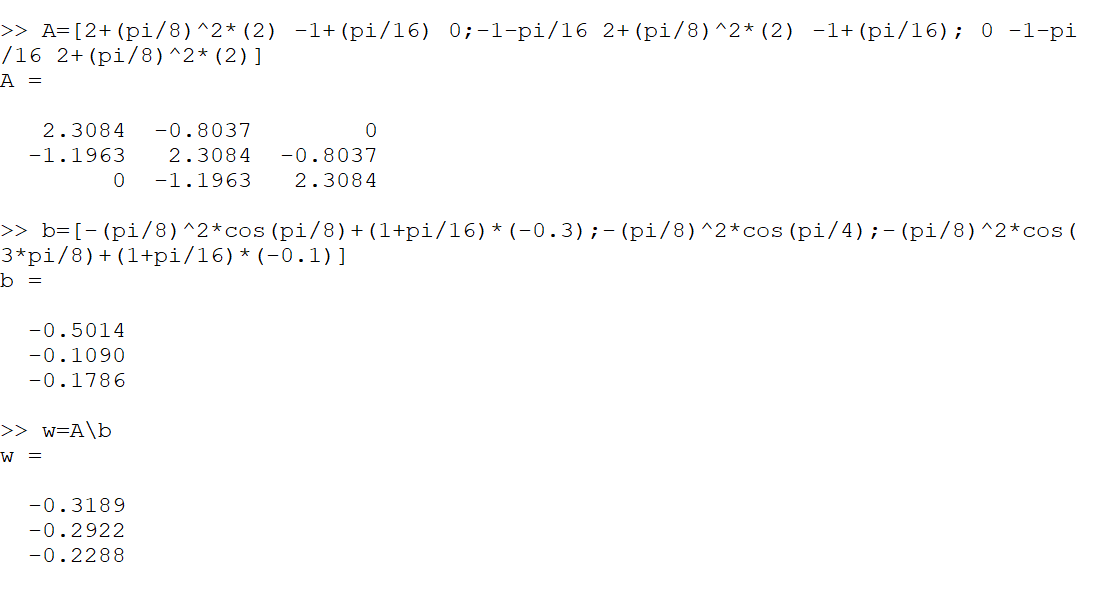
\includegraphics[scale=0.5]{TerceraUnidad/Codigo_Octave_ResolucionSistemaLineal.png}
\caption{Código ingresado en la ventana de comandos para resolver el sistema $\mathbf{Aw=b}$ en Octave}
\end{figure}
\end{frame}
\end{comment}


%===================================
\begin{frame}{Ejemplo 2}
\begin{block}{Ejercicio tomado de un examen de reposición del IIPA2022}
Dada la ecuación diferencial 
$$y''+ey'-e^xy=e, \quad 0\leq x \leq 1, \quad y(0)=0, \quad y(1)=0$$
usando el método de diferencias finitas con $h=0.25$
\end{block}
Primero, reescribimos la ecuación diferencial como sigue:
$$y''=-ey'+e^xy+e$$
Por lo tanto, 
\begin{displaymath}
\begin{array}{l}
p(x)=-e\\
q(x)=e^x\\
r(x)=e
\end{array}
\end{displaymath}
Considerando a $h=0.25$, en el intervalo $0\leq x \leq 1$ se hace la partición con los puntos:
$$x_0=0 \qquad x_1=0.25 \qquad x_2=0.5 \qquad x_3=0.75 \qquad x_4=1$$
\end{frame}

%===================================
\begin{frame}
Dado que se conoce el valor exacto de $y$ en la frontera, es decir en $x_0$ y $x_4$. Se desea encontrar una aproximación de la solución en los 3 puntos restantes de la partición: 
\begin{displaymath}
\begin{array}{r}
y(x_1)=y(0.25)\approx w_1\\
y(x_2)=y(0.50)\approx w_2\\
y(x_3)=y(0.75)\approx w_3
\end{array}
\end{displaymath}
Aplicando el método de diferencias finitas obtenemos el sistema $\mathbf{Aw=b}$ asiguiente:
\begin{displaymath}
\mathbf{A}=\begin{pmatrix}
2+\bigg(\dfrac{1}{4}\bigg)^2(e^{0.25}) & & -1+\dfrac{\frac{1}{4}}{2}(-e) & &0\\ 
-1-\dfrac{\frac{1}{4}}{2}(-e) && 2+\bigg(\dfrac{1}{4}\bigg)^2(e^{0.5}) & &-1+\dfrac{\frac{1}{4}}{2}(-e) \\
0 & & -1-\dfrac{\frac{1}{4}}{2}(-e) && 2+\bigg(\dfrac{1}{4}\bigg)^2(e^{7.5})
\end{pmatrix}
\end{displaymath}
\end{frame}

%=====================================
\begin{frame}
\begin{displaymath}
\mathbf{b}=
\begin{pmatrix}
-\bigg(\dfrac{1}{4}\bigg)^2(e)+\bigg(1+\dfrac{\frac{1}{4}}{2}(-e)\bigg)(0)\\
-\bigg(\dfrac{1}{4}\bigg)^2(e)\\
-\bigg(\dfrac{1}{4}\bigg)^2(e)+\bigg(1-\dfrac{\frac{1}{4}}{2}(-e)\bigg)(0)
\end{pmatrix}
\end{displaymath}
Resolviendo el sistema, se obtiene:
\begin{displaymath}
\mathbf{w}=\begin{pmatrix}
w_1\\
w_2\\
w_3
\end{pmatrix}
=
\begin{pmatrix}
-0.250242\\
-0.261738\\
-0.160728
\end{pmatrix}
\end{displaymath}
\end{frame}